\chapter{Аналитический раздел}
\section{Объекты сцены}
Сцена состоит из следующих объектов:
\begin{itemize}
	\item вулкан --- эффузивное геологическое образование, имеющее кратер, из которого вулканические газы поступают на поверхность из недр планеты. Основной объект сцены;
	\item источник света на бесконечности --- источник света для задания фонового освещения;
	\item стол тефры --- дисперсная масса, выбрасываемая из жерла вулкана при извержении.
\end{itemize}

\section{Способы задания модели трехмерных объектов}

\subsection{Каркасная}
Модель состоит из вершин и ребер, без данных о внутренних точках поверхностей, ограниченных этими ребрами.\cite{lit2}.

\subsection{Поверхностная}
Поверхность объекта может быть представлена либо аналитическими выражениями, либо полигональной сеткой. Данная модель описывает исключительно внешние геометрические характеристики, такие как форма и границы, но не включает сведения о внутреннем строении и не определяет, где относительно поверхности расположен материал.\cite{lit2}.

\subsection{Объемная}
Поверхность каждого объекта представлена как непрерывная и математически описываемая. Такая модель полностью характеризует трёхмерную форму и включает данные о материале, из которого создан объект. Также содержится информация о направлении внутренней нормали, что позволяет определить расположение материала относительно поверхности.\cite{lit2}.


Для визуализации вулкана была выбрана поверхностная модель, в связи с распространенностью STL моделей, являющихся поверхностными, для представления реально существующего ландшафта земной поверхности.

\section{Алгоритмы закраски}

\subsection{Простой алгоритм закраски}

В простом алгоритме закраски интенсивность цвета определяется для всего полигона на основе внешней нормали к его поверхности с использованием закона Ламберта. При таком алгоритме закраски граница между полигонами получается четко выраженной. Данный метод закраски используется в случаях, когда применение более продвинутых алгоритмов ведет к сильному увеличению вычислительной сложности.

\subsection{Закраска Гуро}
Метод Гуро основывается на интерполяции интенсивности света, при которой разные точки на грани получают различные значения освещенности. Для этого вычисляются нормали в каждой вершине грани, а затем значения интенсивности интерполируются между точками смежных граней. Нормали для граней определяются в первую очередь, затем нормали в вершинах рассчитываются как среднее значение нормалей прилегающих граней. На основе этих нормалей вычисляются значения интенсивности с учетом выбранной модели отражения света, после чего полигоны граней закрашиваются с учетом линейной интерполяции интенсивности в вершинах.

Этот метод эффективно работает для небольших граней, находящихся далеко от источника света. Однако, когда грань становится достаточно большой, расстояние от источника света до её центра будет меньше, чем до вершин, что должно привести к более яркому освещению центра. Из-за линейной интерполяции, применяемой в методе, этого эффекта не удается достичь, что приводит к неестественному распределению освещенности на некоторых участках грани.\cite{lit2}.

\subsection{Закраска Фонга}
Метод закраски по Фонгу использует интерполяцию векторов нормалей вместо простой интерполяции интенсивности вдоль сканирующей строки. Это позволяет точно моделировать кривизну поверхности и создавать изображения с высокой реалистичностью. Такой подход особенно эффективен для симуляции зеркальных отражений, поскольку он обеспечивает плавные переходы освещенности и высокую детализацию. В результате метод Фонга минимизирует эффект полос на поверхностях и создает более гладкие и детализированные переходы света, что способствует получению естественного и детализированного изображения.

Для визуализации вулкана был выбран простой метод закраски,~т.~к. модель представлена большим числом полигонов, для которых определены только нормали к поверхности. Вычисление нормалей к вершинам полигонов и интерполяция цвета приводят к значительному увеличению вычислений и замедлению визуализации.
 
\section{Алгоритмы удаления невидимых линий и поверхностей}

\subsection{Алгоритм Робертса} 

Алгоритм Робертса является первым известным методом удаления невидимых линий и работает в объектном пространстве. Он предназначен для обработки выпуклых объектов и выполняет удаление рёбер и граней, экранируемых самим телом. Далее оставшиеся видимые рёбра каждого объекта сравниваются со всеми другими объектами сцены, чтобы определить, какие их части оказываются перекрытыми. Метод обладает вычислительной сложностью, возрастающей пропорционально квадрату числа объектов.\cite{lit2}.

\subsection{Алгоритм Варнока}
Алгоритм работает в контексте изображения, выполняя анализ содержимого окна. Его задача --- определить, является ли окно пустым или слишком сложным для визуализации. В случае, если содержимое окна слишком детализировано, алгоритм рекурсивно разделяет окно на более мелкие сегменты, пока каждый из них не станет достаточно простым для отображения или не достигнет минимального разрешения. Основным недостатком такого метода является увеличение вычислительных затрат и сложности из-за использования рекурсии, что может привести к замедлению обработки изображений с высоким уровнем детализации.\cite{lit2}.

\subsection{Алгоритм z – буфера}
Этот алгоритм для удаления невидимых поверхностей является одним из базовых. Он функционирует в пространстве изображения, расширяя концепцию буфера кадра. Буфер кадра используется для хранения атрибутов (например, интенсивности) каждого пикселя на изображении. Вместе с буфером кадра используется Z-буфер, представляющий собой специализированную память для хранения координат Z (глубины) каждого видимого пикселя. В процессе работы глубина нового пикселя, который требуется добавить в буфер кадра, сравнивается с глубиной пикселя, уже записанного в Z-буфер. Если новый пиксель находится ближе к наблюдателю, чем тот, который уже находится в буфере, его значения добавляются в буфер кадра, и Z-буфер обновляется соответствующей глубиной. Если же новый пиксель дальше, то никаких изменений не происходит. Таким образом, алгоритм для каждой точки (x, y) вычисляет максимальное значение функции Z(x, y).\cite{lit2}.


\subsection{Алгоритм трассировки лучей}
В этом методе для каждого пикселя на изображении определяется ближайшая грань, к которой этот пиксель относится. Для этого через пиксель направляется луч, который пересекает все грани, и из этих пересечений выбирается ближайшее. Алгоритм трассировки лучей включает несколько шагов. Сначала необходимо найти уравнение луча, который проходит через рассматриваемый пиксель и точку взгляда наблюдателя. Вычисляется точка пересечения этого луча с ближайшим объектом сцены. После этого пиксель закрашивается цветом объекта, с которым луч пересекся, и процесс продолжается для следующего пикселя. В случае, если пересечений с объектами нет, пиксель закрашивается цветом фона, и алгоритм переходит к следующему пикселю. Трассировка лучей учитывает процессы отражения, преломления и прохождения через поверхности объектов, заканчиваясь, когда луч встречает непрозрачный объект, который виден наблюдателю. 
\cite{lit2}.

Для моделирования вулкана был выбран Z-буфер,~т.~к. метод позволяет эффективно работать с объектами, представленными большим числом полигонов, например, реальными горными ландшафтами.

\section{Анализ моделей освещения}
\subsection{Модель Ламберта}
Модель Ламберта является одной из простейших моделей освещения, в которой учитывается только идеальное диффузное отражение света от поверхности. В этой модели предполагается, что свет, падающий на точку поверхности, равномерно рассеивается во всех направлениях полупространства, и освещенность в точке зависит лишь от плотности света в этой точке. Освещенность линейно зависит от косинуса угла падения света, при этом положение наблюдателя не имеет значения, так как диффузно отраженный свет равномерно рассеивается во всех направлениях.

Основной закон, описывающий диффузное отражение, — это закон косинусов Ламберта, который утверждает, что интенсивность отраженного света пропорциональна косинусу угла падения света на поверхность. Этот закон выражается следующим уравнением:
\begin{equation}
	I = I_l k_d \cos(\theta),
\end{equation}
где:  
\begin{itemize}
	\item $I$ — интенсивность отраженного света,  
	\item $I_l$ — интенсивность падающего света от точечного источника,  
	\item $k_d$ — коэффициент диффузного отражения,  
	\item $\theta$ — угол между направлением падающего света $L$ и нормалью к поверхности $N$.  
\end{itemize}

Закон может быть также представлен в виде, использующем нормированный вектор нормали к поверхности и нормированный вектор направления падающего луча света:

\begin{equation}
	I = I_l \cdot (L \cdot N)
\end{equation}


\subsection{Модель Фонга}

Модель освещения Фонга сочетает три компонента: фоновое освещение, диффузное рассеяние и зеркальное отражение. Модель Фонга представляет собой комбинированную модель освещения, которая учитывает как диффузное, так и зеркальное отражение света, а также фоновое освещение. Она особенно полезна для моделирования ярких блестящих объектов, так как зеркальное отражение вызывает появление световых бликов на поверхностях с высокой степенью отражения, таких как металлы или влага.

Коэффициент зеркального отражения в модели Фонга зависит от угла падения света. Даже при перпендикулярном падении света только часть энергии отражается зеркально, а остальная часть либо поглощается, либо рассеивается диффузно. Эти соотношения зависят от материала поверхности и длины волны света. Например, для различных материалов (металлы, стекло, матовые поверхности) коэффициенты отражения будут различаться, что влияет на видимость бликов и отражений.

Формула модели освещения Фонга:
\begin{equation}
I = I_a \cdot K_a + I_d \cdot K_d \cdot (L \cdot N) + I_s \cdot K_s \cdot (R \cdot V)^n.
\end{equation}

Модель Ламберта учитывает только диффузное отражение света, что подходит для визуализации горной поверхности, которая имеет матовую структуру и рассеивает свет в разных направлениях.

\section{Алгоритм для визуализации поведения газов}
Уравнения Навье---Стокса описывают движение газа и жидкости, и могут быть использованы для моделирования различных физических процессов, включая генерацию дыма. Для симуляции дыма в рамках уравнений Навье-Стокса необходимо учитывать динамику потока воздуха и взаимодействие частиц дыма с окружающей средой.

Математически состояние дыма в данный момент времени моделируется как векторное поле скорости, которое назначает вектор скорости каждой точке в пространстве. Для визуализации дыма, в том числе в контексте извержения вулкана, можно применить математическую модель, основанную на уравнениях Навье---Стокса, которая описывает изменение векторного поля скорости во времени. Уравнение~\ref{eq:first_Navie_Stocks} этой модели дает точное описание того, как скорость жидкости или газа будет изменяться в зависимости от действующих сил, что важно для создания визуальных эффектов дыма. При этом, поскольку общих решений уравнений Навье-Стокса не существует, подход предложенный Дж. Стэмом~\cite{stam} предполагает упрощенное восприятие этих уравнений и использование метода Гаусса---Зейделя для решения СЛАУ~\cite{lit3, Gauss}.

\begin{equation}
	\label{eq:first_Navie_Stocks}
	\frac{\partial \vec{u}}{\partial t} = - (\vec{u} \cdot \nabla) \vec{u} + \nu \nabla^2 \vec{u} + f
\end{equation}
где:
\begin{itemize}
	\item $u$ --- вектор скорости жидкости или газа;
	\item $\frac{\partial \vec{u}}{\partial t}$ --- изменение скорости по времени;
	\item $(\vec{u} \cdot \nabla) \vec{u}$ --- нелинейный член, описывающий изменение скорости из-за движения жидкости;
	\item \(\nu \nabla^2 \vec{u}\) --- вязкость (диффузия);
	\item \(\vec{f}\) -- внешние силы (например, гравитация, теплоотдача).
\end{itemize}
	
В контексте визуализации дыма, особенно при моделировании извержений вулканов, необходимо моделировать движение частиц, связанных с потоком горячих газов и пепла. Поскольку моделирование каждой частицы дыма требует значительных вычислительных ресурсов, эффективным решением является использование плотности дыма --- непрерывной функции, которая определяет количество частиц в каждой точке пространства. Изменение плотности через поле скорости жидкости или газа может быть описано с использованием уравнения~\ref{eq:second_Navie_Stoks}, аналогичного уравнению для скорости, но с упрощением, поскольку модель плотности является линейной, в отличие от нелинейности модели скорости. Для визуализации дымовых эффектов, в том числе при моделировании вулканических извержений, модель плотности дыма используется для расчета того, как частицы будут распространяться в пространстве, учитывая изменения в потоке горячих газов и пепла. Визуализация достигается путем отображения плотности дыма в различных точках, что позволяет создать реалистичные эффекты подъема и распространения дыма, характерные для извержений вулканов. 

\begin{equation}
	\label{eq:second_Navie_Stoks}
	\frac{\partial \rho}{\partial t} = -(\vec{u} \cdot \nabla) \rho + \kappa \nabla^2 \rho + S
\end{equation}
где:
\begin{itemize}
	\item \(\rho\) --- плотность жидкости или газ;
	\item \((\vec{u} \cdot \nabla) \rho\) --- изменение плотности дыма из-за потока жидкости или газа;
	\item \(\kappa \nabla^2 \rho\) --- диффузия дыма (влияние турбулентности или молекулярной диффузии);
	\item \(S\) --- источник дыма (например, извержение вулкана, где горячие газы и пепел выбрасываются в атмосферу).
\end{itemize}

Таким образом необходимо сначала вычислить изменение поля скорости за заданный промежуток времени. Вычисления производятся в порядке, обратно порядку слагаемых, в правой части уравнения~\ref{eq:first_Navie_Stocks}: в первую очередь добавляются источники поля, т.~e. внешние силы; затем вычисляется рассеяние поля с учетом вязкости среды; после чего - самоадвекция поля скорости, т.~e. перенос поля под действием себя же. При этом в расчете самоадвекции необходимо учесть закон сохранения массы~\cite{stam}.

После обновления поля скорости, вычисляется изменение распределения плотности дыма в пространстве, аналогично вычислению изменения поля скорости. Обработка слагаемых в уравнении~\ref{eq:second_Navie_Stoks} вновь производится в обратном порядке: добавляются источники дыма с высокой начальной плотностью, которая в дальнейшем будет перенесена полем скорости; после этого вычисляется диффузия дыма; наконец вычисляется адвекция плотности дыма полем скорости. Так как к этому моменту для поля скорости выполняется закон сохранения массы, использовать его при вычислении изменения распределения плотности нет необходимости. Пример для двухмерной симуляции представлен на рисунке~\ref{fig:diffusion}.


\begin{figure}[H]
	\centering
	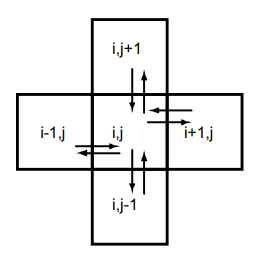
\includegraphics[width=0.5\textwidth, page=1]{assets/img/diffusion.png}   
	\caption{Пример диффузии для двумерной симуляции}
	\label{fig:diffusion}
\end{figure}

В обоих случаях под диффузией предполагается обмен ячейки ограничивающего параллелепипеда плотностью или скоростью с соседними по граням ячейками.  

\section*{Вывод}
Была выбрана поверхностная модель для визуализации вулкана. Для удаления невидимых линий и поверхностей выбран алгоритм использующий z-буфер. Был рассмотрен алгоритм для визуализации поведение газов.
